%!TEX root = ../../main.tex
\chapter{The Nonlinear Surface Susceptibility}\label{chap:chi2}
\partialtoc


In recent years surface nonlinear optical spectroscopies, particulary surface
second-harmonic generation (SSHG), have evolved as useful nondestructive and
noninvasive tools to study surface and interface properties. These properties
include atomic structure, phase transitions, adsorption of atoms, and many
others.\cite{daumPRL93, mcgilpOE94, meyerPRL95, powerPRL95, godefroyAPL96,
hoferAPA96, dadapPRB97, bloembergenAPB99, mcgilpSRL99, suzukiAPB99,
mitchellSS01, hughesPRB96, guyotPRB88, downerPSSA01, shenAPB99, shenNAT89,
chenPRL81, mendozaPRL98, downerSIA01} Nowadays, SSHG spectroscopy is a crucial
tool for research and development in microelectronics,
\cite{zheltikovLP00} semiconductors, \cite{lupkeSSR99} nanomaterials,
\cite{salazar-aparicioPRB14} and many more recent areas of great scientific and
commercial interest.\cite{cazzanelliNM14} The high surface sensitivity of SSHG
spectroscopy is due to the fact that within the dipole approximation the bulk
SHG signal of centrosymmetric materials is identically zero. However, the SHG
process can occur only at the surface where the inversion symmetry is broken.
The bulk quadrupole contribution for centrosymmetric materials is different from
zero, but usually it is very small \cite{downerSIA01}, and could be neglected.
Much of the foundation of surface science has been built from experiments
involving emission or scattering of electrons from surfaces. These require
ultrahigh vacuum (UHV) environments and provide no access to buried interfaces.
However, SSHG is compatible with non-UHV conditions and has access to interfaces
buried beneath transparent overlayers. Even when applied to surfaces in UHV, the
light source and detectors can be aligned and used outside the vacuum chamber.

The usefulness of SSHG could be limited by the lack of microscopic theoretical
understanding of the nonlinear spectra. The macroscopic phenomenological theory
of SSHG, which relates the intensity, phase, and polarization of detected fields
to nonlinear and linear susceptibilities at the material interface is now fully
developed.\cite{downerSIA01} However, microscopic theory that relates
electronic-level structure to the nonlinear source polarization is still being
developed. \cite{butcherPOPS63, aspnesPRB72, sipePRB93, levinePRB94,aversaPRB95,
hughesPRB96, rashkeevPRB98,beyond} Within the independent particle approximation
(IPA) some frameworks for bulk SHG have been developed to study the nonlinear
optical response of bulk materials. \cite{butcherPOPS63, aspnesPRB72, sipePRB93,
levinePRB94,aversaPRB95, hughesPRB96, rashkeevPRB98} In this thesis we put
forward an approach to calculate the microscopic second-harmonic surface
susceptibility that encompasses several theoretical features not taken into
account before in the case of a surface.

The most used framework for \textit{ab initio} calculations, Density Functional
Theory (DFT) within the Local Density Approximation (LDA),
\cite{kohnPR65} underestimates the energy band gap of semiconductors. It is well
understood that one has to include the many-body interaction to correct for this
underestimation of the gap. In this context, the so-called GW
approximation\cite{onidaRMP02} is known to correct the electronic gap of most
semiconductors\cite{luceroJPCM12}. However this can be a very expensive
calculation and thus one uses the much simpler scissors operator scheme.
\cite{levinePRL89,levinePRL91,delsolePRB93} This allows us to ``open'' the
DFT-LDA gap to its correct experimental or GW value for most bulk
semiconductors. This approximation has already been used in linear optical
calculations for surfaces,\cite{kippPRL96} thus improving the agreement with
experimental results. In this context, to correct for the underestimation of the
energy band gap of semiconductors Nastos et al.\cite{nastosPRB05} used the
``length gauge'' or ``$\mathbf{r}\cdot\mathbf{E}$'' gauge to show how to
correctly include the many-body corrections through the scissors operator in the
SH susceptibility. Later, Cabellos \textit{et al}.\cite{cabellosPRB09}
elaborated a derivation of the ``velocity gauge'' or
``$\mathbf{A}\cdot\mathbf{v}$'' gauge properly including the scissors operator
and proved gauge invariance with respect to the length gauge. From these works
it is clear the length gauge is a much better starting point to obtain the
surface SH (SSH) susceptibility, as will be elaborated in this thesis. However,
these considerations are only valid for bulk semiconductors.

Concerning the optical response of surfaces and interfaces, Reining \textit{et
al.}\cite{reiningPRB94} introduced the concept of a cut function in order to
obtain the surface SH susceptibility tensor. This cut function is required since
one usually uses a slab approach when treating semi-infinite surface
systems.\cite{reiningPRB94} If the slab is centrosymmetric the susceptibility
tensor will be identically zero. The cut function is such that it separates the
nonlinear response for the two surfaces of the slab avoiding the destructive
interference between them giving a finite value that one identifies with the SSH
susceptibility tensor. If the slab is not centrosymmetric the cut function can
be used to separate the different signals coming from either surface of the
slab. Indeed, one of the main results of this thesis is to show that the SSH
susceptibility tensor obtained by using the cut function is correctly extracted
from the slab. After Reining \textit{et al.},\cite{reiningPRB94} Refs.
\cite{mendozaPRL98,arzatePRB01,mendozaPRB01,mejiaPRB02,sanoPRB02} followed upon
this work and in particular Ref. \cite{arzatePRB01} went into a detailed
analysis of the different contributions to the SHG spectra of a surface and the
nuanced relationship between bulk, surface, interband, intraband, $1\omega$ and
$2\omega$ terms, and Ref. \cite{mejiaRMF04} developed a layer-by-layer analysis
for the nonlinear responses of semiconductor systems, within a tight-binding
framework. This model allows for obtaining results from selected regions of a
system including the surface. However, in these references the scissors operator
is either excluded or incorrectly implemented. In the works that include this
operator,  the velocity gauge was used to derive the expressions for
$\chi^{\mathrm{abc}}(-2\omega;\omega,\omega)$. Nevertheless, a term in the
time-dependent perturbation scheme necessary to satisfy the gauge invariance of
$\chi^{\mathrm{abc}}(-2\omega;\omega,\omega)$  was omitted. This was
demonstrated in Ref. \cite{cabellosPRB09} where a comparison between the
velocity and the length gauge was carried out.

Finally, DFT-LDA calculations are often based on the use of pseudopotentials. As
it will be discussed in this thesis, the presence of a nonlocal part of the
pseudopotential introduces corrections to the momentum operator of the electron
that have to be included with care in the SSH susceptibility. For the bulk
counterpart see for instance Refs. \cite{ismailPRL01,luppiPRB08}.

Therefore, within the IPA the most complete approach for the calculation of the
SSH susceptibility is one which includes (i) the scissors correction, (ii) the
contribution of the nonlocal part of the pseudopotential, and (iii) the cut
function. Therefore, the goal of this paper is to derive a new expression within
the length gauge for the SSH susceptibility tensor
$\chi^{\mathrm{a}\mathrm{b}\mathrm{c}}(-2\omega;\omega,\omega)$ that includes
the aforementioned contributions. The inclusion of these three contributions
makes our scheme unprecedented and opens the possibility to study surface SHG
with more versatility and providing accurate results.


%%%%%%%%%%%%%%%%%%%%%%%%%%%%%%%%%%%%%%%%%%%%%%%%%%%%%%%%%%%%%%%%%%%%%%%%%%%%%%%%
%%%%%%%%%%%%%%%%%%%%%%%%%%%%%%%%%%%%%%%%%%%%%%%%%%%%%%%%%%%%%%%%%%%%%%%%%%%%%%%%

\section{The nonlinear surface susceptibility}

In this section I will outline the general procedure to obtain the surface
susceptibility tensor for SHG. We start with the nonlinear polarization
$\mathbf{P}(\mathbf{r})$ of a bulk system, written as
\begin{equation}\label{mshg}
\begin{split}
P^{\mathrm{a}}(\mathbf{r},2\omega)
= \chi^{\mathrm{abc}}(-2\omega;\omega,\omega)
  E^{\mathrm{b}}(\mathbf{r},\omega)E^{\mathrm{c}}(\mathbf{r},\omega)
+ \chi^{\mathrm{abcd}}(-2\omega;\omega,\omega)
  E^{\mathrm{b}}(\mathbf{r},\omega)\nabla^{\mathrm{c}}
  E^{\mathrm{d}}(\mathbf{r},\omega)
+ \cdots,
\end{split}
\end{equation}
where $\chi^{\mathrm{abc}}(-2\omega;\omega,\omega)$ and
$\chi^{\mathrm{abcd}}(-2\omega;\omega,\omega)$ correspond to the dipolar and
quadrupolar susceptibility tensors, and $\mathbf{E}(\mathbf{r})$ is the incoming
electric field along the different Cartesian directions denoted by the roman
superscripts. For ease of notation, I will drop the $\omega$ arguments from this
point on.
% The sum continues with higher multipolar terms.
At this point I introduce the units of the quantities above. For simplicity, we
use the MKS system of units. The units of $\mathbf{E}(\mathbf{r})$ are
$[\mathbf{E}] = $ V/m, and the units of $\mathbf{P}(\mathbf{r})$ are
$[\mathbf{P}] = $ V/m since $\mathbf{P}(\mathbf{r})$ is a \emph{bulk}
polarization. Therefore, the units of the bulk $\chi^{\mathrm{abc}}$ are
$[\chi^{\mathrm{abc}}] = $ m/V.

If we consider a semi-infinite system with a centrosymmetric bulk, we can obtain
a bulk and a surface nonlinear polarization that differ from each other from
symmetry considerations alone. To show this, we take
\begin{equation}\label{mshg2}
P^{\mathrm{a}}(\mathbf{r})
= \chi^{\mathrm{abc}}E^{\mathrm{b}}(\mathbf{r})E^{\mathrm{c}}(\mathbf{r})
+ \chi^{\mathrm{abcd}}E^{\mathrm{b}}(\mathbf{r})
  \frac{\partial}{\partial\mathbf{r}^{\mathrm{c}}}E^{\mathrm{d}}(\mathbf{r}) 
+ \cdots,
\end{equation}
as the polarization with respect to the $\mathbf{r}$ coordinate system, and 
\begin{equation}\label{mshg3}
P^{\mathrm{a}}(-\mathbf{r})
= \chi^{\mathrm{abc}}E^{\mathrm{b}}(-\mathbf{r})E^{\mathrm{c}}(-\mathbf{r})
+ \chi^{\mathrm{abcd}}E^{\mathrm{b}}(-\mathbf{r})
  \frac{\partial}{\partial(-\mathbf{r}^{\mathrm{c}})}E^{\mathrm{d}}(-\mathbf{r}) 
+ \cdots, 
\end{equation}
as the polarization in the inverted coordinate system, where we take
$\mathbf{r}$ to $-\mathbf{r}$. Note that we have kept the same susceptibility
tensors as they must be invariant under $\mathbf{r} \to -\mathbf{r}$ since the
system is centrosymmetric. Recalling that $\mathbf{P}(\mathbf{r})$ and
$\mathbf{E}(\mathbf{r})$ are polar vectors
\cite{jacksonbook}, we have that Eq. \eqref{mshg3} reduces to
\begin{align}\label{mshg4}
-P^{\mathrm{a}}(\mathbf{r})
&= \chi^{\mathrm{abc}}(-E^{\mathrm{b}}(\mathbf{r}))(-E^{\mathrm{c}}(\mathbf{r}))
 + \chi^{\mathrm{abcd}}(-E^{\mathrm{b}}(\mathbf{r}))
(-\frac{\partial}{\partial\mathbf{r}^{\mathrm{c}}})(-E^{\mathrm{d}}(\mathbf{r})) 
 + \cdots,\nonumber\\
P^{\mathrm{a}}(\mathbf{r})
&= -\chi^{\mathrm{abc}}E^{\mathrm{b}}(\mathbf{r})E^{\mathrm{c}}(\mathbf{r})
 + \chi^{\mathrm{abcd}}E^{\mathrm{b}}(\mathbf{r})
   \frac{\partial}{\partial\mathbf{r}^{\mathrm{c}}}E^{\mathrm{d}}(\mathbf{r}) 
 + \cdots,
\end{align}
that when compared with Eq. \eqref{mshg2} leads to the conclusion that
\begin{equation}\label{sshg}
\begin{split}
\chi^{\mathrm{abc}} &= 0,\\
&\qquad\qquad\text{(centrosymmetric bulk)}\\
\chi^{\mathrm{abcd}} &\ne 0,
\end{split}
\end{equation}
for a centrosymmetric bulk.

The surface of a centrosymmetric system necessarily breaks the centrosymmetry;
thus, there are no symmetry restrictions imposed on the $\chi^{\mathrm{abc}}$
produced from the surface region. Therefore, it is convenient to define the
surface nonlinear polarization $\mathbf{P}_{\mathrm{surface}}$ as follows,
\begin{equation}\label{sshgp}
P^{\mathrm{a}}_{\mathrm{surface}}
\equiv \chi^{\mathrm{abc}}_{\mathrm{surface}}E^{\mathrm{b}}E^{\mathrm{c}},
\end{equation}
where $\chi^{\mathrm{abc}}_{\mathrm{surface}}$ is the surface nonlinear
susceptibility. In this case, the units of $[\mathbf{P}_{\mathrm{surface}}]$ are
V, and $[\chi^{\mathrm{abc}}_{\mathrm{surface}}]$ are m$^{2}$/V. The
contribution from $\chi^{\mathrm{abcd}}$ to the surface polarization is
neglected as it originates from a higher order multipole. From Eq. \eqref{mshg}
we have that for the bulk of a semi-infinite system,
\begin{equation}\label{sshgp3}
P^{\mathrm{a}}_{\mathrm{bulk}}
= \chi^{\mathrm{abcd}}_{\mathrm{bulk}}
  E^{\mathrm{b}}\nabla^{\mathrm{c}}E^{\mathrm{d}},  
\end{equation}
which is the bulk nonlinear polarization; in this case the dipolar contribution
$\chi^{\mathrm{abc}}_{\mathrm{bulk}} = 0$ since we are in the centrosymmetric
bulk. Note that the surface nonlinear polarization is of dipolar electric order
while the bulk polarization is of quadrupolar electric and dipolar magnetic
order \cite{bloembergenPR62}. The surface
$\chi^{\mathrm{abc}}_{\mathrm{surface}}$ and bulk
$\chi^{\mathrm{abcd}}_{\mathrm{bulk}}$ susceptibilities are tensors of rank
three and four, respectively.

In this work, we will only concentrate on SSHG, even though bulk-generated SH is
also a very important optical phenomenon. To this end, we will neglect the
contribution from Eq. \eqref{sshgp3} and only consider the surface term from Eq.
\eqref{sshgp}. I will also exclude other interesting surface SH phenomena like,
electric field induced second-harmonic (EFISH), which would be represented by a
surface susceptibility tensor of quadrupolar origin. As mentioned in Chapter
\ref{chap:intro}, in centrosymmetric systems for which the quadrupolar bulk
response is much smaller than the dipolar surface response, SH is a very capable
and powerful optical surface probe \cite{downerSIA01}.

In the following sections of this chapter, we show the theoretical
approach to derive the expressions for the surface susceptibility tensor
$\chi^{\mathrm{abc}}_{\mathrm{surface}}$.

\begin{figure}[t]
\centering
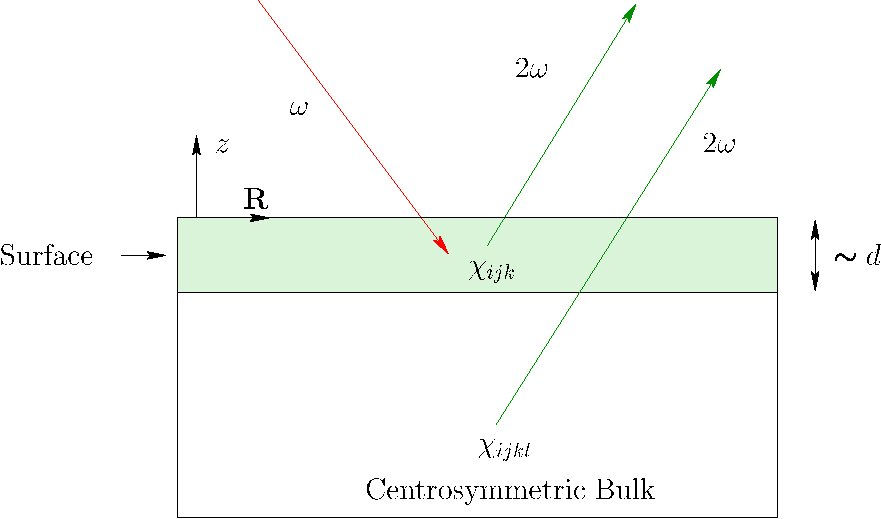
\includegraphics[scale=0.6]{content/figures/diag-system}
\caption{Sketch of a semi-infinite system with a centrosymmetric bulk. The
surface region is of width $\sim d$. The incoming photon of frequency $\omega$
is represented by a downward red arrow, whereas both the surface and bulk
created second-harmonic photons of frequency $2\omega$ are represented by upward
green arrows. The red color suggests an incoming infrared photon with a green
second-harmonic photon. The dipolar ($\chi^{\mathrm{abc}}_{\mathrm{surface}}$),
and quadrupolar ($\chi^{\mathrm{abcd}_{\mathrm{bulk}}}$) susceptibility tensors
are shown in the regions where they are nonzero. The $z$-axis is perpendicular
to the surface and $\mathbf{R}$ is parallel to it.}
\label{fsystem}
\end{figure}


%%%%%%%%%%%%%%%%%%%%%%%%%%%%%%%%%%%%%%%%%%%%%%%%%%%%%%%%%%%%%%%%%%%%%%%%%%%%%%%%
%%%%%%%%%%%%%%%%%%%%%%%%%%%%%%%%%%%%%%%%%%%%%%%%%%%%%%%%%%%%%%%%%%%%%%%%%%%%%%%%

\section{Time-dependent Perturbation Theory}\label{tdpt}

We assume the IPA, a classical electromagnetic field, and quantum mechanical
matter. We neglect local field and excitonic effects. We can describe the system
using the one electron density operator ${\rho}$, with which we can calculate
the expectation value of a single-particle observable $\mathcal{O}$ as
\begin{equation}\label{traza}
\left\langle\mathcal{O}\right\rangle
= \mathrm{Tr}(\rho\mathcal{O}),
\end{equation}
with $\mathcal{O}$ the associated quantum mechanical operator and Tr the 
trace. The density operator satisfies
\begin{equation}\label{eqrho}
i\hbar \frac{d\rho}{dt} = \left[H,\rho\right],
\end{equation}
with $H(t)$ as the total single electron Hamiltonian, written as 
\begin{equation*}
H(t) = H_{0} + H_{I}(t),  
\label{achea}
\end{equation*}
where $H_{0}$ is the unperturbed time-independent Hamiltonian, and $H_{I}(t)$ is
the time-dependent potential energy due to the interaction of the electron with
the electromagnetic field. To proceed with the solution of $\rho$ it is
convenient to use the interaction picture, where a unitary operator
\begin{equation}\label{ou}
U = e^{iH_{0}t/\hbar},
\end{equation}
transforms any operator $\mathcal{O}$ into
\begin{equation}\label{ip}
\tilde{\mathcal{O}} = U\mathcal{O}U^{\dagger}.
\end{equation}
Even if $\mathcal{O}$ is time-independent, $\tilde{\mathcal{O}}$ is
time-dependent through the explicit time dependence of $U$. The dynamical
equation for $\tilde{\rho}$ is given by
\begin{equation}\label{intrho}
i\hbar \frac{d\tilde{\rho}}{dt}
= \left[-e\mathbf{r}_{I}(t)\cdot\mathbf{E}(t),\tilde{\rho}\right]
= [\tilde{H}_{I}(t), \tilde{\rho}],
\end{equation}
with solution 
\begin{equation}\label{intrho2}
i\hbar \tilde{\rho}(t)
= i\hbar \tilde{\rho}_{0} + 
\int_{-\infty}^{t}
\left[\tilde{H}_{I}(t^{\prime}),\tilde{\rho}(t^{\prime})\right]\,dt^{\prime},  
% \label{trans}
\end{equation}
where $\tilde{\rho}_{0} = \tilde{\rho}(t = -\infty)$ is the unperturbed density
matrix.

We assume that the interaction is switched-on adiabatically and choose a
time-periodic perturbing field, to write
\begin{equation}\label{efield}
\mathbf{E}(t)
= \mathbf{E} e^{-i\omega t}e^{\eta t}
= \mathbf{E} e^{-i\tilde{\omega} t},
\end{equation}
with
\begin{equation}\label{got}
\tilde{\omega} =\omega + i\eta,
\end{equation} 
where $\eta > 0$ assures that at $t = -\infty$, the interaction is zero and has
its full strength $\mathbf{E}$ at $t = 0$. After computing the required time
integrals one takes $\eta\to 0$. Also, $\tilde{\rho}(t = -\infty)$ should be
time independent and thus $[\tilde{H}_{I},\tilde{\rho}]_{t = -\infty} = 0$. This
implies that $\tilde{\rho}(t = -\infty)\equiv\tilde{\rho}_{0}$, such that
\begin{equation}\label{nrhon}
\langle n\mathbf{k}\vert \tilde{\rho}_{0} \vert m\mathbf{k}'\rangle
= f_{n}(\hbar\omega^{\Sigma}_{n}(\mathbf{k}))
\delta_{nm}\delta(\mathbf{k}-\mathbf{k}'),
\end{equation}
with $f_{n}(\hbar\omega^{\Sigma}_{n}(\mathbf{k})) = f_{n}$ as the Fermi-Dirac
distribution function. For a clean, cold semiconductor $f_{n}=1$ when $n$ is a
valence ($v$) or occupied band, and zero when $n$ is a conduction ($c$) or empty
band. We assume this for the remainder of this work. As we neglect spin-orbit
coupling, the final expression for $\chi^{\mathrm{abc}}(-2\omega;\omega,\omega)$
has to be multiplied by a factor of 2 to account for spin-degeneracy. The
expectation values must always satisfy $\langle\mathcal{O}\rangle =
\mathrm{Tr}({\rho}\mathcal{O}) = Tr(\tilde{\rho}\tilde{\mathcal{O}})$.

We solve Eq. \eqref{intrho2} using the standard iterative
solution, for which we write
\begin{equation}\label{rhop}
\tilde{\rho}
= \tilde{\rho}^{(0)}
+ \tilde{\rho}^{(1)}
+ \tilde{\rho}^{(2)}
+ \cdots,
\end{equation}
where $\tilde{\rho}^{(N)}$ where the superscript denotes the order (power) with
which each term depends on the perturbation $H_{I}(t)$. Then, Eq.
\eqref{intrho2} reads
\begin{equation}\label{intrho3}
  \tilde{\rho}^{(0)} 
+ \tilde{\rho}^{(1)} 
+ \tilde{\rho}^{(2)} 
+ \cdots
= \tilde{\rho}_{0}
+ \frac{1}{i\hbar}\int_{-\infty}^{t} 
  \left[
  \tilde{H}_{I}(t'),\tilde{\rho}^{(0)}+\tilde{\rho}^{(1)}+\tilde{\rho}^{(2)}
  + \cdots
  \right]\,dt',
\end{equation}
where, by equating equal orders in the perturbation, we find
\begin{equation}\label{rho0}
\tilde{\rho}^{(0)}\equiv\tilde{\rho}_{0},
\end{equation}
and the $N$th-order term
\begin{equation}\label{rhoN}
\tilde{\rho}^{(N)}(t)=
\frac{1}{i\hbar}
\int_{-\infty}^{t}
\left[\tilde{H}_{I}(t'),\tilde{\rho}^{(N-1)}(t')\right]\,dt'.
\end{equation}
It is simple to show that matrix elements of Eq. (\ref{rhoN}) satisfy 
$\langle n\mathbf{k}| \rho^{(N+1)}(t) |m\mathbf{k}'\rangle =
\rho^{(N+1)}_{nm}(\mathbf{k})\delta(\mathbf{k}-\mathbf{k}')$, with
\begin{equation}\label{rtilde}
\rho^{(N+1)}_{nm}(\mathbf{k};t)
= \frac{e}{i\hbar}\int_{-\infty}^t
\langle n\mathbf{k}|
\left[\mathbf{r}_{I}(t'),\tilde{\rho}^{(N)}(t')\right]
|m\mathbf{k}\rangle
\cdot\mathbf{E}(t')dt'.
\end{equation}
This shows that the $N + 1$ solution is determined by the $N$th solution, which
in turn is determined by the $N - 1$ solution, and so on. Starting from the
zeroth order solution given in Eq. \eqref{rho0}, we can solve for any desired
order.

We will look for the expectation value of the microscopic current density,
$\mathbf{J}$, given by
\begin{equation*}
\mathbf{J} = \langle{\mathbf{J}}\rangle 
           = \frac{e}{A}\mathrm{Tr}({\rho}\dot{\mathbf{r}}),
\end{equation*}
where $\dot{\mathbf{r}}$ is the time derivative of the position operator of the
electron with charge $e$, defined as
\begin{equation}
\mathbf{v}\equiv \dot{\mathbf{r}}=\frac{1}{i\hbar }[\mathbf{r},H_0],  
\label{mv}
\end{equation}
with $\mathbf{v}$ the velocity operator of the electron, and $A$ the area of the
unit cell. We calculate the polarization density $\mathbf{P}$, related to
$\mathbf{J}$ by $\mathbf{J}=d\mathbf{P}/dt$. We write the second-order nonlinear
polarization as,
\begin{equation}
\boldsymbol{\mathcal{P}}^{\mathrm{a}}(2\omega)=
\chi^{\mathrm{abc}}(-2\omega;\omega,\omega)
E^{\mathrm{b}}(\omega)E^{\mathrm{c}}(\omega),  
\label{pshg}
\end{equation}
where $\chi^{\mathrm{a}\mathrm{b}\mathrm{c}}(-2\omega ;\omega ,\omega )$ is the
nonlinear susceptibility responsible for surface second-harmonic generation
(SSHG). The superscripts in Eq.~\eqref{pshg} denote Cartesian components, and if
repeated are to be summed over. Without loss of generality we will define
$\chi^{\mathrm{a}\mathrm{b}\mathrm{c}}(-2\omega;\omega,\omega)$ to satisfy
intrinsic permutation symmetry,
$\chi^{\mathrm{a}\mathrm{b}\mathrm{c}}(-2\omega;\omega ,\omega )
=\chi^{\mathrm{a}\mathrm{c}\mathrm{b}}(-2\omega ;\omega,\omega )$.

The unperturbed Hamiltonian is used to solve the Kohn-Sham equations
\cite{kohnPR65} of Density Functional Theory (DFT). It is convenient to work
within the Local Density Approximation (LDA), so we label the hamiltonian with
the corresponding LDA superscript. Any other approximation can be used (like the
generalized gradient approximation) and our derivation remains the same. Then,
\begin{equation}\label{ache.2}
H^{\mathrm{LDA}}_{0}(\mathbf{r},\mathbf{p})
= \frac{p^{2}}{2m_e}+V(\mathbf{r},\mathbf{p})
\end{equation}
with $m_e$ the mass of the electron, $\mathbf{p}=-i\hbar\boldsymbol{\nabla}$ its
canonical momentum, and $V$ the periodic crystal potential, where we neglect
spin-orbit terms. To be more general in our derivation of
$\chi^{\mathrm{a}\mathrm{b}\mathrm{c}}(-2\omega;\omega,\omega)$, we assume
contribution as is customary for most pseudopotentials, and then we replace $V$
with
\begin{equation}
V^{\mathrm{ps}}(\mathbf{r},\mathbf{p})
= V(\mathbf{r})+V^{\mathrm{nl}}(\mathbf{r},\mathbf{p}),
\end{equation}
where $V(\mathbf{r})$ and $V^{\mathrm{nl}}(\mathbf{r},\mathbf{p})$ are the local
and nonlocal parts, respectively. The argument $(\mathbf{r},\mathbf{p})$ is
equivalent to the explicit $(\mathbf{r},\mathbf{r}')$ nonlocal notation
\cite{ismailPRL01}. For this nonlocal part, we have that
\begin{align}\label{ache.3n}
V^{\mathrm{nl}}(\mathbf{r},\mathbf{r}')\equiv
\langle\mathbf{r}\vert
V^{\mathrm{nl}}
\vert\mathbf{r}'\rangle \neq 0 
\quad\text{for}\quad\mathbf{r} \neq \mathbf{r}',
\end{align}
where $V^{\mathrm{nl}}(\mathbf{r},\mathbf{r}')$ is a function of $\mathbf{r}$
and $\mathbf{r}'$ representing the nonlocal contribution of the pseudopotential.
In case of a local potential, i.e. $V= V(\mathbf{r})$, like that of all-electron
schemes, we simply omit the contribution of
$V^{\mathrm{nl}}(\mathbf{r},\mathbf{p})$ from the results that we have derived.

It is well known that the use of the LDA leads to an underestimation of the band
gap. A standard procedure to correct for this is to use the ``scissors
approximation'', where the conduction bands are rigidly shifted in energy so
that the band gap corresponds to the accepted experimental electronic band
gap.\cite{levinePRL89,levinePRL91,delsolePRB93} This is often in fairly good
agreement with the GW band gap based on a more sophisticated
calculation.\cite{hybertsenPRB86} The LDA wave functions are used since they
produce band structures with dispersion relations similar to those predicted by
the GW. Mathematically, the scissors (non-local) operator $S$ is added to the
unperturbed or unscissored Hamiltonian $H^{\mathrm{LDA}}_{0}$ ,
\begin{equation}\label{ache.1}
H^\Sigma_{0}(\mathbf{r},\mathbf{p})
= H^{\mathrm{LDA}}_{0}(\mathbf{r},\mathbf{p})
+ S(\mathbf{r},\mathbf{p})
\end{equation}
where 
\begin{equation}\label{hats}
S(\mathbf{r},\mathbf{p}) = \hbar \Delta\sum_{n}\int (1-f_{n})
|n\mathbf{k}\rangle\langle n\mathbf{k}|\,d^{3}k,
\end{equation}
with $\hbar\Delta$ the rigid ($\mathbf{k}$-independent) energy correction to be
applied. The unscissored and scissored Hamiltonians satisfy
\begin{align*}
H^{\mathrm{LDA}}_{0}(\mathbf{r},\mathbf{p})\psi _{n\mathbf{k}}(\mathbf{r}) &=
\hbar \omega^{\mathrm{LDA}}_{n}(\mathbf{k})\psi _{n\mathbf{k}}(\mathbf{r}),
\label{hamils} \\
H_{0}^\Sigma (\mathbf{r},\mathbf{p})\psi _{n\mathbf{k}}(\mathbf{r}) &=
\hbar \omega_{n}^\Sigma(\mathbf{k})\psi _{n\mathbf{k}}(\mathbf{r}),
\end{align*}
where the scissor-shifted energies, $\omega_{n}^\Sigma(\mathbf{k})$, are given
by
\begin{equation}\label{chon.78}
\omega_{n}^\Sigma(\mathbf{k})
= \omega^\mathrm{LDA}_{n}(\mathbf{k})+(1-f_{n})\Delta.
\end{equation}
Lastly, the Schr\"odinger equation reads
\begin{align}\label{ache.4} 
\left(
\frac{-\hbar^2}{2m_{e}}\nabla^{2}
+ V(\mathbf{r})
\right)
\psi_{n\mathbf{k}}(\mathbf{r})
+ \int V^{\mathrm{nl}}(\mathbf{r},\mathbf{r}')
  \psi_{n\mathbf{k}}(\mathbf{r}')\,d\mathbf{r}'
= E_{i}\psi_{n\mathbf{k}}(\mathbf{r}),
\end{align} 
where $\psi_{n\mathbf{k}}(\mathbf{r}) = \langle\mathbf{r}|n\mathbf{k}\rangle =
e^{i\mathbf{k}\cdot\mathbf{r}}u_{n\mathbf{k}}(\mathbf{r})$, are the real space
representations of the Bloch states $|n\mathbf{k}\rangle$ labeled by the band
index $n$ and the crystal momentum $\mathbf{k}$, and
$u_{n\mathbf{k}}(\mathbf{r})$ is cell periodic. We emphasize that the scissored
and unscissored Hamiltonian have the same eigenfunctions.


%%%%%%%%%%%%%%%%%%%%%%%%%%%%%%%%%%%%%%%%%%%%%%%%%%%%%%%%%%%%%%%%%%%%%%%%%%%%%%%%
%%%%%%%%%%%%%%%%%%%%%%%%%%%%%%%%%%%%%%%%%%%%%%%%%%%%%%%%%%%%%%%%%%%%%%%%%%%%%%%%

\section{Length Gauge}\label{longi}

According to Ref. \cite{ismailPRL01}, we first start with the interaction
Hamiltonian expressed in the velocity gauge, containing the nonlocal parts
$V^{nl}(\mathbf{r},\mathbf{p})$ and $S (\mathbf{r},\mathbf{p})$. Within the
dipole approximation and using a gauge transformation, it can be transformed
into an effective Hamiltonian \cite{valerie}
\begin{equation}
H_{I}(t)=-e\mathbf{r}\cdot \mathbf{E}(t).
\label{rde}
\end{equation}
The treatment of the position operator $\mathbf{r}$ for extended Bloch states is
problematic and has been discussed in Refs. \cite{adamsJCP53, blountSSP62}.

{\color{red}
We now work out the commutator of Eq. \eqref{rtilde}. Then,
\begin{align}\label{conmu1}
\langle n\mathbf{k}|
\left[\mathbf{r}_{I}(t),\tilde{\rho}^{(N)}(t)\right]
|m\mathbf{k}\rangle
%%%%%%%%%%%%%%%%%%%%%%%%%%%%%%%%%%%%%%%%%%%%%%%%%%%%%%%%
&= \langle n\mathbf{k}|
\left[U\mathbf{r}U^\dagger,U\rho^{(N)}(t)U^\dagger\right]
|m\mathbf{k}\rangle\nonumber \\
%%%%%%%%%%%%%%%%%%%%%%%%%%%%%%%%%%%%%%%%%%%%%%%%%%%%%%%%
&= \langle n\mathbf{k}|
U\left[\mathbf{r},\rho^{(N)}(t)\right]U^\dagger
|m\mathbf{k}\rangle\\
%%%%%%%%%%%%%%%%%%%%%%%%%%%%%%%%%%%%%%%%%%%%%%%%%%%%%%%%
&= e^{i\omega^\Sigma_{nm\mathbf{k}}t}
\left(
\langle n\mathbf{k}|
  \left[\mathbf{r}_{e},\rho^{(N)}(t)\right]
+ \left[\mathbf{r}_{i},\rho^{(N)}(t)\right]
|m\mathbf{k}\rangle
\right)\nonumber,
\end{align}
where the time dependence of the operator in the interaction picture is
explicitly shown by the exponential factor, and the implicit dependence of
$\rho^{(N)}$ inherited from Eq. \eqref{eqrho} is given through the $t$ argument.
We calculate the interband term first, so using Eq. \eqref{chon.98} we obtain
\begin{align}\label{conmu2}
\langle n\mathbf{k}|
[\hat{\mathbf{r}}_e,\tilde{\rho}^{(N)}(t)]
|m\mathbf{k}\rangle
&=
\sum_{\ell}
\left(
\langle n\mathbf{k}|
\hat{\mathbf{r}}_e
|\ell\mathbf{k}\rangle
\langle \ell\mathbf{k}|
\tilde{\rho}^{(N)}(t)
|m\mathbf{k}\rangle
-
\langle n\mathbf{k}|
\tilde{\rho}^{(N)}(t)
|\ell\mathbf{k}\rangle
\langle \ell\mathbf{k}|
\hat{\mathbf{r}}_e
|m\mathbf{k}\rangle
\right)
\nonumber \\
&=
\sum_{\ell\ne n,m}
\left(
\mathbf{r}_{n\ell}(\mathbf{k})
\rho^{(N)}_{\ell m}(\mathbf{k};t)
-
\rho^{(N)}_{n\ell}(\mathbf{k};t)
\mathbf{r}_{\ell m}(\mathbf{k})
\right)
\nonumber\\
&\equiv
\mathbf{R}^{(N)}_e(\mathbf{k};t)
,
\end{align}
and from Eq. \eqref{conmri3n},
\begin{equation}\label{conmri4}
\langle n\mathbf{k}|
[\hat{\mathbf{r}}_i,\tilde{\rho}^{(N)}(t)]
|m\mathbf{k}'\rangle
=i \delta(\mathbf{k}-\mathbf{k}') (\rho^{(N)}_{nm}(t))_{;\mathbf{k}}
\equiv \delta(\mathbf{k}-\mathbf{k}')\mathbf{R}_i^{(N)}(\mathbf{k};t).
\end{equation}
Then Eq. \eqref{rtilde} becomes
\begin{equation}\label{rtilde2}
\rho^{(N+1)}_{I,nm}(\mathbf{k};t)
=\frac{ie}{\hbar}\int_{-\infty}^t dt'
e^{i(\omega^\Sigma_{nm\mathbf{k}}-\tilde{\omega})t'}
\left[R_e^{\mathrm{b}(N)}(\mathbf{k};t')+R_i^{\mathrm{b}(N)}(\mathbf{k};t')\right]E^{\mathrm{b}}
,
\end{equation}
where the roman superindices
$\mathrm{a},\mathrm{b},\mathrm{c}$ denote Cartesian components that are summed over if repeated.
Starting from the linear response and proceeding from Eq. \eqref{nrhon} and  \eqref{conmu2},
\begin{align}\label{R0e}
R_e^{\mathrm{b}(0)}(\mathbf{k};t)
&=
\sum_{\ell}
\left(
r^{\mathrm{b}}_{n\ell}(\mathbf{k})
\rho^{(0)}_{\ell m}(\mathbf{k})
-
\rho^{(0)}_{n\ell}(\mathbf{k})
r^{\mathrm{b}}_{\ell m}(\mathbf{k})
\right)
\nonumber \\
&=
\sum_{\ell}
\left(
r^{\mathrm{b}}_{n\ell}(\mathbf{k})
\delta_{\ell m}f_m(\hbar\omega^\Sigma_m(\mathbf{k}))
-
\delta_{n\ell}f_n(\hbar\omega^{\Sigma}_{n}(\mathbf{k}))
r^{\mathrm{b}}_{\ell m}(\mathbf{k})
\right)
\nonumber \\
&=
f_{mn\mathbf{k}}
r^{\mathrm{b}}_{nm}(\mathbf{k}),
\end{align}
where $f_{mn\mathbf{k}}=f_{m\mathbf{k}}-f_{n\mathbf{k}}$.
From now on,
it should be clear that the matrix elements of $\mathbf{r}_{nm}$ imply
$n\notin D_m$.
We also have from Eq. \eqref{conmri4} and Eq. \eqref{gendevnn} that
\begin{equation}\label{R0i}
R_i^{\mathrm{b}(0)}(\mathbf{k})
= i(\rho^{(0)}_{nm})_{;k^{\mathrm{b}}}
= i\delta_{nm}(f_{n\mathbf{k}})_{;k^{\mathrm{b}}}
= i\delta_{nm}\nabla_{k^{\mathrm{b}}} f_{n\mathbf{k}}.
\end{equation}
For a semiconductor at $T = 0$, $f_{n\mathbf{k}} = 1$ if the state
$|n\mathbf{k}\rangle$ is a valence state and $f_{n\mathbf{k}} = 0$ if it is a
conduction state. Thus, $\nabla_\mathbf{k} f_{n\mathbf{k}} = 0$,
$\mathbf{R}_i^{(0)} = 0$ and the linear response has no contribution from the
intraband transitions. Then,
\begin{align}\label{rtilde2n}
\rho^{(1)}_{I,nm}(\mathbf{k};t)
&=\frac{ie}{\hbar}
f_{mn\mathbf{k}}
r^{\mathrm{b}}_{nm}(\mathbf{k})E^{\mathrm{b}}
\int_{-\infty}^t dt'
e^{i(\omega^\Sigma_{nm\mathbf{k}}-\tilde{\omega})t'}
\nonumber \\
&=\frac{e}{\hbar}
f_{mn\mathbf{k}}
r^{\mathrm{b}}_{nm}(\mathbf{k})E^{\mathrm{b}}
\frac{e^{i(\omega^\Sigma_{nm\mathbf{k}}-\tilde{\omega})t}}
{\omega^\Sigma_{nm\mathbf{k}}-\tilde{\omega}}
\nonumber \\
&=
e^{i\omega^\Sigma_{nm\mathbf{k}}t}
B^{\mathrm{b}}_{mn}(\mathbf{k})E^{\mathrm{b}}(t)
\nonumber \\
&=
e^{i\omega^\Sigma_{nm\mathbf{k}}t}
\rho^{(1)}_{nm}(\mathbf{k};t)
,
\end{align}
with
\begin{equation}\label{rho1} 
B^{\mathrm{b}}_{nm}(\mathbf{k},\omega)=
\frac{e}{\hbar}
\frac{f_{mn\mathbf{k}}r^{\mathrm{b}}_{nm}(\mathbf{k})}
     {\omega^\Sigma_{nm\mathbf{k}}-\tilde{\omega}},
\end{equation} 
and
\begin{equation}\label{rhonoi1}
\rho^{(1)}_{nm}(\mathbf{k};t)
= B^{\mathrm{b}}_{mn}(\mathbf{k},\omega)E^{\mathrm{b}}(\omega)
  e^{-i\tilde{\omega}t}.
\end{equation}

Now, we calculate the second-order response. Then, from Eq. \eqref{conmu2}
\begin{align}\label{R1e}
R_e^{\mathrm{b}(1)}(\mathbf{k};t)
&=
\sum_{\ell}
\left(
r^{\mathrm{b}}_{n\ell}(\mathbf{k})
\rho^{(1)}_{\ell m}(\mathbf{k};t)
-
\rho^{(1)}_{n\ell}(\mathbf{k};t)
r^{\mathrm{b}}_{\ell m}(\mathbf{k})
\right)
\nonumber \\
&=
\sum_{\ell}
\left(
r^{\mathrm{b}}_{n\ell}(\mathbf{k})
B^{\mathrm{c}}_{\ell m}(\mathbf{k},\omega)
-
B^{\mathrm{c}}_{n\ell}(\mathbf{k},\omega)
r^{\mathrm{b}}_{\ell m}(\mathbf{k})
\right)E^{\mathrm{c}}(t)
,
\end{align}
and from Eq. \eqref{conmri4}
\begin{equation}\label{R1i}
R_i^{\mathrm{b}(1)}(\mathbf{k};t)=
i(\rho^{(1)}_{nm}(t))_{;k^{\mathrm{b}}}=
iE^{\mathrm{c}}(t)(B^{\mathrm{c}}_{nm}(\mathbf{k},\omega))_{;k^{\mathrm{b}}}
.
\end{equation}

Using Eqs. \eqref{R1e} and  \eqref{R1i} in Eq. (\ref{rtilde2}),
we obtain
\begin{align}\label{rtilde33}
\rho^{(2)}_{I,nm}(\mathbf{k};t)
&=
\frac{ie}{\hbar}
\bigg[
\sum_{\ell}
\Big(
r^{\mathrm{b}}_{n\ell}(\mathbf{k})
B^{\mathrm{c}}_{\ell m}(\mathbf{k},\omega)
-
B^{\mathrm{c}}_{n\ell}(\mathbf{k},\omega)
r^{\mathrm{b}}_{\ell m}(\mathbf{k})
\Big)
+
i
(B^{\mathrm{c}}_{nm}(\mathbf{k},\omega))_{;k^{\mathrm{b}}}
\bigg]
E^{\mathrm{b}}_{\omega}E_{\omega}^{\mathrm{c}}
\int_{-\infty}^t dt'
e^{i(\omega^\Sigma_{nm\mathbf{k}}-2\tilde{\omega})t'}
\nonumber \\
&=
\frac{e}{\hbar}
\bigg[
\sum_{\ell}
\Big(
r^{\mathrm{b}}_{n\ell}(\mathbf{k})
B^{\mathrm{c}}_{\ell m}(\mathbf{k},\omega)
-
B^{\mathrm{c}}_{n\ell}(\mathbf{k},\omega)
r^{\mathrm{b}}_{\ell m}(\mathbf{k})
\Big)
+
i
(B^{\mathrm{c}}_{nm}(\mathbf{k},\omega))_{;k^{\mathrm{b}}}
\bigg]
E^{\mathrm{b}}_{\omega}E_{\omega}^{\mathrm{c}}
\frac{e^{i(\omega^\Sigma_{nm\mathbf{k}}-2\tilde{\omega})t}}
{\omega^\Sigma_{nm\mathbf{k}}-2\tilde{\omega}}
\nonumber \\
&=
e^{i\omega^\Sigma_{nm\mathbf{k}}t}
\rho_{nm}^{(2)}(\mathbf{k};t)
.
\end{align}
Now, we write
$\rho_{nm}^{(2)}(\mathbf{k};t)=\rho_{nm}^{(2)}(\mathbf{k};2\omega)e^{-i2\tilde{\omega} t}$,
with
\begin{align}\label{rho2}
\rho_{nm}^{(2)}(\mathbf{k};2\omega)&=\frac{e}{i\hbar}\frac{1}{\omega^\Sigma_{nm\mathbf{k}}-2\tilde{\omega}}
\bigg[-(B_{nm}^{\mathrm{c}}(\mathbf{k},\omega)_{;k^{\mathrm{b}}}
+i\sum_\ell\Big(r_{n\ell}^{\mathrm{b}}B_{\ell m}^{\mathrm{c}}(\mathbf{k},\omega) - B_{n\ell}^{\mathrm{c}}(\mathbf{k},\omega)
  r_{\ell m}^{\mathrm{b}}\Big)
\bigg] 
E^{\mathrm{b}}(\omega)E^{\mathrm{c}}(\omega)
\end{align} 
where $B_{\ell m}^{\mathrm{a}}(\mathbf{k},\omega)$ are given by Eq.
\eqref{rho1}. We remark that $\mathbf{r}_{nm}(\mathbf{k})$  are the same whether
calculated with the LDA or the scissored Hamiltonian (see Eq. \eqref{chon.10}).
We chose the former in this thesis.}

We can take $\hbar\Delta = E_{g} -
E_{g}^\mathrm{LDA}$ where $E_{g}$ is the experimental or GW band gap taken at
the $\Gamma$ point, i.e. $\mathbf{k} = 0$. We used the fact that $\vert
n\mathbf{k}\rangle^\mathrm{LDA} \approx \vert n\mathbf{k}\rangle^\Sigma$, thus
negating the need to label the Bloch states with the LDA or $\Sigma$
superscripts.
{\color{red} Check for reference from Pulci}
The matrix elements of $\mathbf{r}$ are split between the
\emph{intraband} ($\mathbf{r}_{i}$) and \emph{interband} ($\mathbf{r}_{e}$)
parts, where $\mathbf{r} = \mathbf{r}_{i} + \mathbf{r}_{e}$
\cite{adamsJCP53, blountSSP62}, and its matrix elements are \cite{aversaPRB95}
\begin{align}\label{rnminn}
\langle n\mathbf{k}\vert \hat{\mathbf{r}}_{i} |m\mathbf{k}'\rangle 
&= \delta_{nm}
\left[
  \delta(\mathbf{k} - \mathbf{k}')\boldsymbol{\xi}_{nn}(\mathbf{k})
+ i\nabla_{\mathbf{k}}\delta(\mathbf{k} - \mathbf{k}')
\right],\\
\langle n\mathbf{k}| \hat{\mathbf{r}}_{e} |m\mathbf{k}'\rangle 
&= (1- \delta_{nm})\delta(\mathbf{k}-\mathbf{k}')
   \boldsymbol{\xi}_{nm}(\mathbf{k}),\label{rnmenn}
\end{align}
with
\begin{equation}\label{zetann}
\boldsymbol{\xi}_{nm}(\mathbf{k})
\equiv i\frac{(2\pi)^3}{\Omega}
\int_{\Omega}u^{*}_{n\mathbf{k}}(\mathbf{r})
\nabla_{\mathbf{k}}\,u_{m\mathbf{k}}(\mathbf{r})
\,d\mathbf{r},
\end{equation}
where $\Omega$ is the unit cell volume. The interband part, $\mathbf{r}_{e}$,
can be obtained as follows. We start by introducing the velocity operator
\begin{align}\label{vop}
\hat{\mathbf{v}}^{\Sigma} &=
\frac{1}{i\hbar}\left[\hat{\mathbf{r}},\hat{H}^{\Sigma}_{0}\right],
\end{align}
and calculating its matrix elements
\begin{equation}\label{conhrnm}
i\hbar\langle n\mathbf{k}\vert\mathbf{v}^\Sigma\vert m\mathbf{k}\rangle
= \langle n\mathbf{k}\vert
\left[
\hat{\mathbf{r}}, \hat{H}^{\Sigma}_{0}
\right]
  \vert m\mathbf{k}\rangle
= \langle n\mathbf{k}\vert
\hat{\mathbf{r}}\hat{H}^{\Sigma}_{0} - \hat{H}^{\Sigma}_{0}\hat{\mathbf{r}}
\vert m\mathbf{k}\rangle
=
\left(
\hbar\omega^{\Sigma}_{m}(\mathbf{k}) - \hbar\omega^{\Sigma}_{n}(\mathbf{k})
\right)
\langle n\mathbf{k}\vert\hat{\mathbf{r}}\vert m\mathbf{k}\rangle.
\end{equation}
Defining $\omega^\Sigma_{nm}(\mathbf{k}) =
\omega^{\Sigma}_{n}(\mathbf{k}) - \omega^\Sigma_m(\mathbf{k})$, we get
\begin{equation}\label{pmnrmn}
\mathbf{r}_{nm}(\mathbf{k})
= \frac{\mathbf{v}^\Sigma_{nm}(\mathbf{k})}{i\omega^\Sigma_{nm}(\mathbf{k})}
\qquad n\notin D_{m},
\end{equation} 
which can be identified as
$\mathbf{r}_{nm}=(1-\delta_{nm})\boldsymbol{\xi}_{nm}\to \mathbf{r}_{e,nm}$.
Here, $D_m$ are all the possible degenerate $m$-states. When $\mathbf{r}_{i}$
appears in commutators we use \cite{aversaPRB95}
\begin{equation}\label{conmri3n}
\langle n\mathbf{k}\vert
\left[
\hat{\mathbf{r}}_{i}, \hat{\mathcal{O}}
\right]
\vert m\mathbf{k}'\rangle
= i\delta(\mathbf{k} - \mathbf{k}')(\mathcal{O}_{nm})_{;\mathbf{k}},
\end{equation}  
with
\begin{equation}\label{gendevnn}
(\mathcal{O}_{nm})_{;\mathbf{k}} =
  \nabla_{\mathbf{k}}\mathcal{O}_{nm}(\mathbf{k})
- i\mathcal{O}_{nm}(\mathbf{k})
\left(
\boldsymbol{\xi}_{nn}(\mathbf{k}) - \boldsymbol{\xi}_{mm}(\mathbf{k})
\right),
\end{equation} 
where ``$;\mathbf{k}$'' denotes the generalized derivative (see Appendix
\ref{app:re_ri}).

As can be seen from Eq. \eqref{ache.1} and \eqref{ache.2}, both $\mathcal{S}$
and $\hat{V}^{\mathrm{nl}}$ are nonlocal potentials. Their contribution in the
calculation of the optical response has to be considered in order to get
reliable results \cite{ismailPRL01}. We proceed as follows: from Eqs.
\eqref{vop}, \eqref{ache.1} and \eqref{ache.2} we find
\begin{align}\label{vop2}
\hat{\mathbf{v}}^{\Sigma} &=
\frac{\hat{\mathbf{p}}}{m_{e}} + \frac{1}{i\hbar}
\left[\hat{\mathbf{r}},\hat{V}^{\mathrm{nl}}(\mathbf{r},\mathbf{r}')\right]
+ \frac{1}{i\hbar}
  \left[\hat{\mathbf{r}},\hat{\mathcal{S}}(\mathbf{r},\mathbf{p})\right]
\nonumber\\
&\equiv
  \hat{\mathbf{v}} + \hat{\mathbf{v}}^{\mathrm{nl}} 
+ \hat{\mathbf{v}}^{\mathcal{S}}
= \hat{\mathbf{v}}^\mathrm{LDA} + \hat{\mathbf{v}}^{\mathcal{S}},
\end{align}
where we have defined
\begin{equation}\label{conhr}
\begin{split}
\hat{\mathbf{v}} &=\frac{\hat{\mathbf{p}}}{m_{e}}\\
\hat{\mathbf{v}}^{\mathrm{nl}} &= \frac{1}{i\hbar}
  \left[\hat{\mathbf{r}},\hat{V}^{\mathrm{nl}}\right]\\
\hat{\mathbf{v}}^{\mathcal{S}} &= \frac{1}{i\hbar}
  \left[\hat{\mathbf{r}},\hat{S}(\mathbf{r},\mathbf{p})\right]\\
\hat{\mathbf{v}}^\mathrm{LDA} &= \hat{\mathbf{v}}+\hat{\mathbf{v}}^{\mathrm{nl}}
\end{split}
\end{equation}  
with $\hat{\mathbf{p}}= -i\hbar\boldsymbol{\nabla}$ the momentum operator. Using
Eq. \eqref{hats}, we obtain that the matrix elements of
$\hat{\mathbf{v}}^{\mathcal{S}}$ are given by
\begin{equation}\label{chon.2} 
\mathbf{v}^{\mathcal{S}}_{nm} = i\Delta f_{mn}\mathbf{r}_{nm},
\end{equation}
with $f_{nm} = f_{n} - f_{m}$, where we see that $\mathbf{v}^{\mathcal{S}}_{nn}
= 0$, then
\begin{align}\label{chon.8}
\mathbf{v}^\Sigma_{nm} 
&= \mathbf{v}^\mathrm{LDA}_{nm} + i\Delta f_{mn}\mathbf{r}_{nm}\nonumber\\
&= \mathbf{v}^\mathrm{LDA}_{nm} + i\Delta f_{mn}
   \frac{\mathbf{v}^\Sigma_{nm}(\mathbf{k})}{i\omega^\Sigma_{nm}(\mathbf{k})}
   \nonumber\\
%%%%%%%%%%%%%%%%%%%%%%%%%%%%%%%%%%%%%%%%%%%%%%%%%
\mathbf{v}^\Sigma_{nm}
  \frac{\omega^\Sigma_{nm}-\Delta f_{mn}}{\omega^\Sigma_{nm}}
&= \mathbf{v}^\mathrm{LDA}_{nm}\nonumber\\
%%%%%%%%%%%%%%%%%%%%%%%%%%%%%%%%%%%%%%%%%%%%%%%%%
\mathbf{v}^\Sigma_{nm}\frac{\omega^{\mathrm{LDA}}_{nm}}{\omega^\Sigma_{nm}}
&= \mathbf{v}^\mathrm{LDA}_{nm}\nonumber\\
%%%%%%%%%%%%%%%%%%%%%%%%%%%%%%%%%%%%%%%%%%%%%%%%%
\frac{\mathbf{v}^\Sigma_{nm}}{\omega^\Sigma_{nm}}
&= \frac{\mathbf{v}^\mathrm{LDA}_{nm}}{\omega^{\mathrm{LDA}}_{nm}},
\end{align}
since $\omega^\Sigma_{nm}-\Delta f_{mn}=\omega^{\mathrm{LDA}}_{nm}$. Therefore,
\begin{align}\label{chon.9}
\begin{split}
\mathbf{v}^\Sigma_{nm}(\mathbf{k}) &=
\frac{\omega^\Sigma_{nm}}{\omega^{\mathrm{LDA}}_{nm}}
\mathbf{v}^\mathrm{LDA}_{nm}(\mathbf{k})
= \left(
1 + \frac{\Delta}{\omega_c(\mathbf{k})-\omega_v(\mathbf{k})}
\right)
\mathbf{v}^\mathrm{LDA}_{nm}(\mathbf{k})\qquad n\notin D_{m}\\\\
\mathbf{v}^\Sigma_{nn}(\mathbf{k}) &= \mathbf{v}^\mathrm{LDA}_{nn}(\mathbf{k}),
\end{split}
\end{align} 
and Eq. \eqref{pmnrmn} gives
\begin{align}\label{chon.10}
\mathbf{r}_{nm}(\mathbf{k})
= \frac{\mathbf{v}^\Sigma_{nm}(\mathbf{k})}{i\omega^\Sigma_{nm}(\mathbf{k})}
= \frac{\mathbf{v}^\mathrm{LDA}_{nm}(\mathbf{k})}
{i\omega^{\mathrm{LDA}}_{nm}(\mathbf{k})} \qquad n\notin D_{m}.
\end{align}
Therefore, the matrix elements of $\mathbf{r}_{e}$ are the same whether we use
the LDA or the scissored Hamiltonian; thus, there is no need to label them
with either LDA or $\Sigma$ superscripts. Thus, we can write
\begin{equation}\label{chon.98}
\mathbf{r}_{e,nm}\to\mathbf{r}_{nm}(\mathbf{k}) =
\frac{\mathbf{v}^\mathrm{LDA}_{nm}(\mathbf{k})}
     {i\omega^{\mathrm{LDA}}_{nm}(\mathbf{k})}
\qquad n\notin D_{m},
\end{equation}   
which gives the interband matrix elements of the position operator in terms of
the matrix elements of $\hat{\mathbf{v}}^\mathrm{LDA}$. These matrix elements
include the matrix elements of $\mathbf{v}^{\mathrm{nl}}_{nm}(\mathbf{k})$ which
can be readily calculated for fully separable nonlocal pseudopotentials in the
Kleinman-Bylander form \cite{mottaCMS10, kleinmanPRL82, adolphPRB96}. In
Appendix \ref{app:vnlme} we outline how this is accomplished.


%%%%%%%%%%%%%%%%%%%%%%%%%%%%%%%%%%%%%%%%%%%%%%%%%%%%%%%%%%%%%%%%%%%%%%%%%%%%%%%%
%%%%%%%%%%%%%%%%%%%%%%%%%%%%%%%%%%%%%%%%%%%%%%%%%%%%%%%%%%%%%%%%%%%%%%%%%%%%%%%%

\section{Layered Current Density}\label{cd}

In this section, we derive the expressions for the microscopic current density
of a given layer in the unit cell of the system. The approach we use to study
the surface of a semi-infinite semiconductor crystal is as follows. Instead of
using a semi-infinite system, we replace it by a slab (see Fig. \ref{fslab}).
The slab consists of a front and back surface, and in between these two surfaces
is the bulk of the system. In general the surface of a crystal reconstructs or
relaxes as the atoms move to find equilibrium positions. This is due to the fact
that the otherwise balanced forces are disrupted when the surface atoms do not
find their partner atoms that are now absent at the surface of the slab.

To take the reconstruction or relaxation into account, we take ``surface'' to
mean the true surface of the first layer of atoms, and some of the atomic
sub-layers adjacent to it. Since the front and the back surfaces of the slab are
usually identical the total slab is centrosymmetric. This implies that
$\chi^{\mathrm{abc}}_{\mathrm{slab}} = 0$, and thus we must find a way to bypass
this characteristic of a centrosymmetric slab in order to have a finite
$\chi^{\mathrm{abc}}_{\mathrm{surface}}$ representative of the surface. Even if the front and
back surfaces of the slab are different, breaking the centrosymmetry and
therefore giving an overall $\chi^{\mathrm{abc}}_{\mathrm{slab}}\ne 0$, we still
need a procedure to extract the front surface $\chi^{\mathrm{abc}}_{\mathrm{front}}$ and the
back surface $\chi^{\mathrm{abc}}_{\mathrm{back}}$ from the nonlinear susceptibility $\chi^{\mathrm{abc}}_{\mathrm{slab}} = \chi^{\mathrm{abc}}_{\mathrm{front}} - \chi^{\mathrm{abc}}_{\mathrm{back}}$ of the
entire slab.

A convenient way to accomplish the separation of the SH signal of either surface
is to introduce a ``cut function'', $\mathcal{C}(z)$, which is usually taken to be
unity over one half of the slab and zero over the other half \cite{reiningPRB94}.
In this case $\mathcal{C}(z)$ will give the contribution of the side of the slab for
which $\mathcal{C}(z)=1$. We can generalize this simple choice for $\mathcal{C}(z)$ by a
top-hat cut function $\mathcal{C}^{\ell}(z)$ that selects a given layer $\ell$,
\begin{equation}
\label{sz}
\mathcal{C}^{\ell}(z)=\Theta(z-z_\ell+\Delta_\ell^{\mathrm{b}})
            \Theta(z_\ell-z+\Delta_\ell^f),
\end{equation}
where $\Theta$ is the Heaviside function. Here, $\Delta_\ell^{f/b}$
is the distance that the $\ell$-th layer extends towards the front
$(f)$ or back $(b)$ from its $z_\ell$ position. 
$\Delta_\ell^f+\Delta_\ell^b$ is the thickness of layer $\ell$ 
(see Fig. \ref{fslab}).
\begin{figure}[b]
\centering
%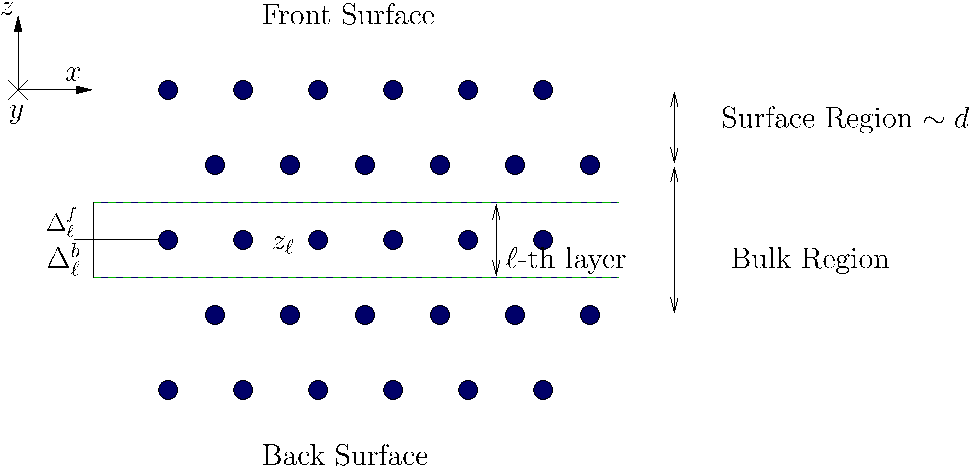
\includegraphics[height=5cm,width=7cm]{slab}
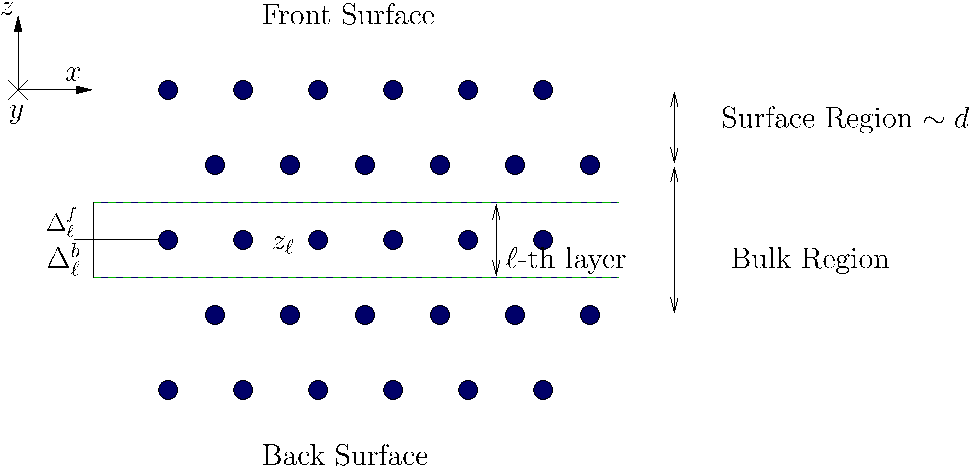
\includegraphics[scale=.7]{content/figures/diag-slab}
\caption{A sketch of a slab where the circles represent atoms.\label{fslab}}
\end{figure}

Now, we show how this ``cut function'' $\mathcal{C}^{\ell}(z)$ is introduced in
the calculation of $\chi^{\mathrm{abc}}$. 
The microscopic current density is given by
\begin{equation}\label{jmic}
\mathbf{j}(\mathbf{r},t)=\mathrm{Tr}(\hat{\mathbf{j}}(\mathbf{r})\tilde{\rho}(t)),
\end{equation}
where the operator for the electron's current is
\begin{equation}\label{hatjmic}
\hat{\mathbf{j}}(\mathbf{r})=\frac{e}{2}\left(\hat{\mathbf{v}}^{\Sigma} |\mathbf{r}\rangle\langle\mathbf{r}|
+ |\mathbf{r}\rangle\langle\mathbf{r}|\hat{\mathbf{v}}^{\Sigma}\right), 
\end{equation}
where $\hat{\mathbf{v}}^{\Sigma}$ is the electron's velocity operator to be dealt
with below. We define
$\hat{\mu} \equiv |\mathbf{r}\rangle\langle\mathbf{r}|$ and use the cyclic invariance of
the trace to write
\begin{align}\label{jmic2}
\mathrm{Tr}(\hat{\mathbf{j}}(\mathbf{r})\tilde{\rho}(t)
&= \mathrm{Tr}(\tilde{\rho}(t)\hat{\mathbf{j}}(\mathbf{r}))
= \frac{e}{2}
\left(
  \mathrm{Tr}(\tilde{\rho}\hat{\mathbf{v}}^{\Sigma}\hat{\mu})
+ \mathrm{Tr}(\tilde{\rho}\hat{\mu}\hat{\mathbf{v}}^{\Sigma})
\right)\nonumber\\
&= \frac{e}{2}\sum_{n\mathbf{k}}
\left(
\langle n\mathbf{k}| \tilde{\rho}\hat{\mathbf{v}}^{\Sigma}\hat{\mu} |n\mathbf{k}\rangle
+ \langle n\mathbf{k}| \tilde{\rho}\hat{\mu}\hat{\mathbf{v}}^{\Sigma} |n\mathbf{k}\rangle
\right)\nonumber\\
&= \frac{e}{2}\sum_{nm\mathbf{k}}\langle n\mathbf{k}|\tilde{\rho} |m\mathbf{k}\rangle
\left(
\langle m\mathbf{k}| \hat{\mathbf{v}}^{\Sigma}|\mathbf{r}\rangle \langle\mathbf{r}|n\mathbf{k}\rangle
+ \langle m\mathbf{k}|\mathbf{r}\rangle \langle\mathbf{r}| \hat{\mathbf{v}}^{\Sigma} |n\mathbf{k}\rangle
\right)
\nonumber\\
\mathbf{j}(\mathbf{r},t)
&= \sum_{nm\mathbf{k}}\rho_{nm}(\mathbf{k};t)\mathbf{j}_{mn}(\mathbf{k};\mathbf{r}),
\end{align}
where
\begin{equation}\label{jmic3}
\mathbf{j}_{mn}(\mathbf{k};\mathbf{r})=
\frac{e}{2}
\left(
\langle m\mathbf{k}| \hat{\mathbf{v}}^{\Sigma} |\mathbf{r}\rangle \langle\mathbf{r}|n\mathbf{k}\rangle
+
\langle m\mathbf{k}|\mathbf{r}\rangle \langle\mathbf{r}| \hat{\mathbf{v}}^{\Sigma} |n\mathbf{k}\rangle
\right),
\end{equation}
are the matrix elements of the microscopic current operator,
and we have used the fact that the matrix elements between states $|n\mathbf{k}\rangle$
are diagonal in $\mathbf{k}$, i.e. proportional to $\delta(\mathbf{k}-\mathbf{k}')$.

Integrating the microscopic current $\mathbf{j}(\mathbf{r},t)$ over
the entire slab gives the averaged microscopic current density. 
If we want the contribution from only one region of the unit cell 
towards the total current, we can integrate $\mathbf{j}({\mathbf r},t)$ 
over the desired region. The contribution to the current density from the
$\ell$-th layer of the slab is given by
{\color{red} $\Omega \rightarrow A$?}
\begin{equation}\label{jsz}
\frac{1}{\Omega}\int d^3r\, \mathcal{C}^{\ell}(z)\, \mathbf{j}(\mathbf{r},t)
 \equiv \mathbf{J}^{\ell}(t),
\end{equation}
where $\mathbf{J}^{\ell}(t)$ is the microscopic current in the
$\ell$-th layer.
Therefore we define
\begin{equation}\label{vcal}
e{\boldsymbol{\mathcal{V}}}^{\Sigma,\ell}_{mn}(\mathbf{k})
\equiv
%\frac{1}{\Omega}
\int d^3r\, \mathcal{C}^{\ell}(z)\,\mathbf{j}_{mn}({\mathbf{k}};\mathbf{r}),
\end{equation}
to write
\begin{equation}\label{jmac}
J_a^{(N,\ell)}(t)=\frac{e}{\Omega}
\sum_{mn\mathbf{k}}
\mathcal{V}^{\Sigma,a,\ell}_{mn}(\mathbf{k})
\rho^{(N)}_{nm}(\mathbf{k};t),
\end{equation}
as the induced microscopic current of the $\ell$-th layer, to order $N$ 
in the external perturbation. The matrix elements of the 
density operator for $N=1,2$ are given by Eqs. \eqref{rho1} and
\eqref{rho2} respectively. 
The Fourier component of microscopic current of Eq. \eqref{jmac} is given by
\begin{equation}\label{jmac2}
J_{\mathrm{a}}^{(N,\ell)}(\omega_3)=\frac{e}{\Omega}
\sum_{mn\mathbf{k}}
\mathcal{V}^{\Sigma,\mathrm{a},\ell}_{mn}(\mathbf{k})
\rho^{(N)}_{nm}(\mathbf{k};\omega_3)
.
\end{equation}
We proceed to give an explicit expression of
$\boldsymbol{\mathcal{V}}^{\Sigma,\ell}_{mn}(\mathbf{k})$.
From
Eqs. \eqref{vcal} and \eqref{jmic3} we obtain
\begin{equation}\label{intj}
{\boldsymbol{\mathcal{V}}}^{\Sigma,\ell}_{mn}({\mathbf k})=
\frac{1}{2}
\int \mathrm{d}^3 r\,
 \mathcal{C}^{\ell}(z)
\bigg[
\langle m\mathbf{k}|\mathbf{v}^\Sigma | \mathbf{r}\rangle
\langle \mathbf{r} | n \mathbf k \rangle +
\langle m\mathbf{k} | \mathbf{r}\rangle
\langle \mathbf{r} | \mathbf{v}^\Sigma | n \mathbf k \rangle\bigg]
,
\end{equation}  
and using the following property
\begin{equation}\label{nl.2}
\langle \mathbf{r} | \hat{\mathbf{v}}^{\Sigma}(\mathbf{r},\mathbf{r}')| n\mathbf{k} \rangle
=\int d^3 r'' \langle\mathbf{r}|\hat{\mathbf{v}}^{\Sigma}(\mathbf{r},\mathbf{r}')|\mathbf{r}''\rangle
\langle\mathbf{r}''|n\mathbf{k}\rangle
=\hat{\mathbf{v}}^{\Sigma}(\mathbf{r},\mathbf{r}'')
\int d^3 r'' \langle\mathbf{r}|\mathbf{r}''\rangle
\langle\mathbf{r}''|n\mathbf{k}\rangle
=\hat{\mathbf{v}}^{\Sigma}(\mathbf{r},\mathbf{r}')
\psi_{n\mathbf{k}}(\mathbf{r})
,
\end{equation}
that stems from the fact that the operator $\mathbf{v}^\Sigma(\mathbf{r},\mathbf{r}')$ does not act on
$\mathbf{r}''$, we can write
\begin{align}\label{nl.3}
\boldsymbol{\mathcal{V}}^{\Sigma,\ell}_{mn}({\mathbf k})
&=
\frac{1}{2}
\int \mathrm{d}^3 r\,
 \mathcal{C}^{\ell}(z)
 \bigg[
\psi_{n\mathbf{k}}(\mathbf{r})
\hat{\mathbf{v}}^{\Sigma *}\psi^{*}_{m\mathbf{k}}(\mathbf{r})
+ 
\psi^*_{m\mathbf{k}}(\mathbf{r})\hat{\mathbf{v}}^{\Sigma}
\psi_{n\mathbf{k}}(\mathbf{r})
\bigg]
\nonumber\\
&=
\int \mathrm{d}^3 r\,
\psi^*_{m\mathbf{k}}(\mathbf{r})
\left[\frac{\mathcal{C}^{\ell}(z) \mathbf{v}^\Sigma +
\mathbf{v}^\Sigma \mathcal{C}^{\ell}(z)}{2}\right]
\psi_{n\mathbf{k}}(\mathbf{r})
\nonumber\\
&=
\int \mathrm{d}^3 r\,
\psi^*_{m\mathbf{k}}(\mathbf{r})
\boldsymbol{\mathcal{V}}^{\Sigma,\ell}
\psi_{n\mathbf{k}}(\mathbf{r})
.
\end{align}
We used the hermitian property of $\mathbf{v}^\Sigma$ and defined
\begin{align}\label{nl.4}
\boldsymbol{\mathcal{V}}^{\Sigma,\ell}
=
\frac{\mathcal{C}^{\ell}(z) \mathbf{v}^\Sigma +
\mathbf{v}^\Sigma \mathcal{C}^{\ell}(z)}{2}
,
\end{align} 
where the superscript $\ell$ is inherited from $\mathcal{C}^{\ell}(z)$ and we
supress the dependance on $z$ from the increasingly crowded notation.  
We see that the replacement
\begin{align}\label{vcali}
\hat{\mathbf{v}}^{\Sigma} \to \hat{\boldsymbol{\mathcal{V}}}^{\Sigma,\ell}=\left[\frac{\mathcal{C}^{\ell}(z) \hat{\mathbf{v}}^{\Sigma} +
\hat{\mathbf{v}}^{\Sigma}\mathcal{C}^{\ell}(z)}{2}\right]
,
\end{align} 
is all that is needed to change the
velocity operator of the electron $\hat{\mathbf{v}}^{\Sigma}$ to the new velocity
operator $\boldsymbol{\mathcal{V}}^{\Sigma,\ell}$ that implicitly takes into account the
contribution of the region of the slab given by $\mathcal{C}^{\ell}(z)$.
From Eq. \eqref{vop2},
\begin{align}\label{vopii}
\boldsymbol{\mathcal{V}}^{\Sigma,\ell}
&=
\boldsymbol{\mathcal{V}}^{\mathrm{LDA},\ell}
+
\boldsymbol{\mathcal{V}}^{\mathcal{S},\ell}
\nonumber\\
\boldsymbol{\mathcal{V}}^{\mathrm{LDA},\ell}
&=
\boldsymbol{\mathcal{V}}^{\ell}
+
\boldsymbol{\mathcal{V}}^{\mathrm{nl},\ell}
=
\frac{1}{m_{e}}
\boldsymbol{\mathcal{P}}^{\ell}
+
\boldsymbol{\mathcal{V}}^{\mathrm{nl},\ell}
.
\end{align}
{\color{red} Add $\ell$ to app:voila}
As shown in Appendix \ref{app:voila}, Eq. \eqref{chon.8} is generalized to
$\boldsymbol{\mathcal{V}}^{\Sigma,\ell}_{nm} =
(\omega^\Sigma_{nm}/\omega^{\mathrm{LDA}}_{nm})
\boldsymbol{\mathcal{V}}^{\mathrm{LDA},\ell}_{nm}$ from which
$\boldsymbol{\mathcal{V}}^{\Sigma,\ell}_{nm}$ can be readily calculated. As a
consistency test we have calculated the matrix elements of
$\boldsymbol{\mathcal{V}}^{\mathrm{LDA},\ell}$ and
$\boldsymbol{\mathcal{V}}^{\mathcal{S},\ell}$ separately, according to the
derivation presented in Appendix \ref{app:calvs}, and confirm that both
approaches yield identical results for $\chi^{\mathrm{abc}}_{\mathrm{surface}}$.

To limit the response to one surface, the equivalent of Eq. \eqref{nl.4} for
$\boldsymbol{\mathcal{V}}^\ell=\boldsymbol{\mathcal{P}}^\ell/m_{e}$ was proposed
in Ref. \cite{reiningPRB94} and later used in Refs. \cite{mendozaPRL98},
\cite{mendozaPRB01}, \cite{sanoPRB02}, and \cite{mejiaRMF04} also in the context
of SHG. The layer-by-layer analysis of Refs. \cite{hoganPRB03} and
\cite{castilloPRB03} used Eq. \eqref{sz}, limiting the current response to a
particular layer of the slab and used to obtain the anisotropic linear optical
response of semiconductor surfaces. However, the first formal derivation of this
scheme is presented in Ref. \cite{mendozaPRB06} for the linear response, and
here in this thesis, for the second harmonic optical response of semiconductors.


\section{Microscopic surface susceptibility}
In this section we obtain the expressions for the 
surface susceptibility tensor $\chi^{\mathrm{abc}}_{\mathrm{surface}}$.
We start with the basic relation $\mathbf{J} = d\mathbf{P}/dt$ 
with $\mathbf{J}$ the current calculated in Sec. \ref{cd}. From Eq. \eqref{jmac2} 
we obtain
\begin{equation}\label{Pjikn}
J^{(2,\ell)\mathrm{a}}(2\omega)=-i2\tilde{\omega} P^{\mathrm{a}}(2\omega)
=\frac{e}{\Omega}
\sum_{mn\mathbf{k}}
\mathcal{V}^{\Sigma,\mathrm{a},\ell}_{mn}(\mathbf{k})
\rho^{(2)}_{nm}(\mathbf{k};2\omega)
,
\end{equation}
and using Eqs. \eqref{rho2} leads to
\begin{align}\label{Pjikn2}
\chi^{\mathrm{abc},\ell}
&=
\frac{ie}{A E^{\mathrm{b}}_1E^{\mathrm{c}}_2 2\tilde{\omega}}
\sum_{mn\mathbf{k}}
\mathcal{V}^{\Sigma,\mathrm{a},\ell}_{mn}(\mathbf{k})
\rho^{(2)}_{nm}(\mathbf{k};2\tilde{\omega})
\nonumber \\
&=
\frac{e^2}{A\hbar2\tilde{\omega}}
\sum_{mn\mathbf{k}}
\frac{\mathcal{V}^{\Sigma,\mathrm{a},\ell}_{mn}(\mathbf{k})}
{\omega^\Sigma_{nm\mathbf{k}}-2\tilde{\omega}}
\bigg[
-(B_{nm}^{\mathrm{c}}(\mathbf{k},\omega))_{;k^{\mathrm{b}}}
+i\sum_\ell\left(r_{n\ell}^{\mathrm{b}}B_{\ell m}^{\mathrm{c}}(\mathbf{k},\omega) -
  B_{n\ell}^{\mathrm{c}}(\mathbf{k},\omega) 
  r_{\ell m}^{\mathrm{b}}\right)
\bigg]
,
\end{align}
which gives the susceptibility of the $\ell$-th layer, where
$\boldsymbol{\mathcal{V}}^\Sigma$ is given in Eq. \eqref{vopii}, where
{\color{red} Remark about the normalization of the calculated $\chi$ in results}
$A=\Omega/d$ is the surface area of the unit cell that characterizes the surface
of the system. Using Eq. \eqref{rho1} we split this equation into two
contributions from the first and second terms on the right hand side,
{\color{red}!!!!CHECK THAT $\ell$ IS NOT USED AS INDEX, AND SWITCH $l$!!!}
\begin{equation}\label{chii}
\chi^{\mathrm{abc},\ell}_{i}
=-\frac{e^3}{A\hbar^22\tilde{\omega}}\sum_{mn\mathbf{k}}
\frac{\mathcal{V}_{mn}^{\Sigma,\mathrm{a},\ell}}{\omega^\Sigma_{nm}-2\tilde{\omega}}
\left(\frac{f_{mn}r_{nm}^{\mathrm{b}}}{\omega^\Sigma_{nm}-\tilde{\omega}}\right)_{;k^{\mathrm{c}}},
\end{equation} 
and 
\begin{equation}\label{chie}
\chi^{\mathrm{abc},\ell}_{e}
=\frac{ie^3}{A\hbar^22\tilde{\omega}}\sum_{\ell mn\mathbf{k}}
\frac{\mathcal{V}_{mn}^{\Sigma,\mathrm{a},\ell}}{\omega^\Sigma_{nm}-2\tilde{\omega}}
\left(
\frac{r_{n\ell}^{\mathrm{c}} r_{\ell m}^{\mathrm{b}} 
f_{m\ell}}{\omega^\Sigma_{\ell m}-\tilde{\omega}}
-\frac{r_{n\ell}^{\mathrm{b}} r_{\ell m}^{\mathrm{c}} 
f_{\ell n}}{\omega^\Sigma_{n \ell}-\tilde{\omega}}
\right),
\end{equation} 
where $\boldsymbol{\chi}^{\ell}_{i}$ is related to intraband transitions and
 $\boldsymbol{\chi}^{\ell}_{e}$ to interband transitions. For the generalized
 derivative in Eq. \eqref{chii} we use the chain rule and the following result
shown in Appendix \ref{app:gwk},
 \begin{align}\label{eli.13}
\left(\omega^\Sigma_{nm}\right)_{;k^{\mathrm{a}}}
=
\left(\omega^{\mathrm{LDA}}_{nm}\right)_{;k^{\mathrm{a}}}
= 
v_{nn}^{\mathrm{LDA},\mathrm{a}}-v_{mm}^{\mathrm{LDA},\mathrm{a}}\equiv\Delta_{nm}^{\mathrm{a}}
,
\end{align} 
to show that
\begin{equation}\label{gene2}
\left(\frac{f_{mn}r_{nm}^{\mathrm{b}}}{\omega^\Sigma_{nm}-\tilde{\omega}}\right)_{;k^{\mathrm{c}}}=
\frac{f_{mn}}{\omega^\Sigma_{nm}-\tilde{\omega}}\left(r_{nm}^{\mathrm{b}}\right)_{;k^{\mathrm{c}}}
-\frac{f_{mn}r_{nm}^{\mathrm{b}}\Delta_{nm}^\mathrm{c}}{(\omega^\Sigma_{nm}-\tilde{\omega})^2}.
\end{equation}

In order to calculate the nonlinear susceptibility of any given layer 
$\ell$ we simply add the above terms $\boldsymbol{\chi}^{\ell}=
\boldsymbol{\chi}_{e}^{\ell} + \boldsymbol{\chi}_{i}^{\ell}$ and 
then calculate the surface susceptibility as 
\begin{equation}\label{chiijksur}
\boldsymbol{\chi}_{\mathrm{surface}} \equiv \sum_{\ell=1}^{N}\boldsymbol{\chi}^{\ell},
\end{equation} 
where $\ell=1$ is the first layer right at the surface, 
and $\ell=N$ is the bulk-like layer (at a distance $\sim d$ from the
surface  as seen in
Fig. \ref{fsystem}), such that 
\begin{equation}\label{chiijksur2}
\boldsymbol{\chi}^{\ell=N}=0,
\end{equation}
in accordance to Eq. \eqref{sshg} valid for a centrosymmetric environment. 
We note that the value of
$N$ is not universal.
This means that the slab needs to have enough atomic layers for 
Eq. \eqref{chiijksur2} 
to be satisfied and to give converged results for $\boldsymbol{\chi}_{\mathrm{surface}}$. 
We can use Eq. \eqref{chiijksur} for
either the front or the back surface.

We can see from the prefactors of Eqs. \eqref{chii} and \eqref{chie} 
that they diverge as $\tilde{\omega}\to 0$. To remove this apparent divergence of 
$\boldsymbol{\chi}^{\ell}$, we perform a partial fraction expansion over $\tilde{\omega}$. 
As shown in Appendix \ref{appv}, we use time-reversal invariance to 
remove these divergences and obtain the following expressions for $\boldsymbol{\chi}^{\ell}$,
\begin{subequations}\label{eq:chis}
\begin{equation}
\mathrm{Im}[\chi^{\mathrm{abc},\ell}_{e,\omega}]= 
\frac{\pi |e|^3}{2\hbar^2}
\int \frac{d^{3}k}{8\pi^3}
\sum_{vc}\sum_{q\neq(v,c)}\frac{1}{\omega^\Sigma_{cv}}
\left[
\frac{\mathrm{Im}[\mathcal{V}^{\Sigma,\mathrm{a},\ell}_{qc}\{r^{\mathrm{b}}_{cv}r^{\mathrm{c}}_{vq}\}]}
{(2\omega^\Sigma_{cv}-\omega^\Sigma_{cq})} 
-\frac{\mathrm{Im}[\mathcal{V}^{\Sigma,\mathrm{a},\ell}_{vq}\{r^{\mathrm{c}}_{qc}r^{\mathrm{b}}_{cv}\}]}
{(2\omega^\Sigma_{cv}-\omega^\Sigma_{qv})}
\right]\delta(\omega^\Sigma_{cv}-\omega),
\end{equation}  
\begin{equation}
\mathrm{Im}[\chi^{\mathrm{abc},\ell}_{i,\omega}]= 
\frac{\pi\vert e\vert^3}{2\hbar^2}
\int \frac{d^{3}k}{8\pi^3}
\sum_{cv}\frac{1}{(\omega^\Sigma_{cv})^{2}}
\left[
\mathrm{Re}\left[\left\{r^{\mathrm{b}}_{cv}\left(\mathcal{V}^{\Sigma,\mathrm{a},\ell}_{vc}\right)_{;k^{\mathrm{c}}}\right\}\right]
+\frac{\mathrm{Re}\left[\mathcal{V}^{\Sigma,\mathrm{a},\ell}_{vc}\left\{r^{\mathrm{b}}_{cv}
\Delta^{\mathrm{c}}_{cv}\right\}\right]}{\omega^\Sigma_{cv}} 
\right]\delta(\omega^\Sigma_{cv}-\omega),
\end{equation}
\begin{equation}
\mathrm{Im}[\chi^{\mathrm{abc},\ell}_{e,2\omega}]= 
-\frac{\pi |e|^3}{2\hbar^2}
\int \frac{d^{3}k}{8\pi^3}
\sum_{vc}\frac{4}{\omega^\Sigma_{cv}}
\left[
\sum_{v'\ne
  v}\frac{\mathrm{Im}[\mathcal{V}^{\Sigma,\mathrm{a},\ell}_{vc}\{r^{\mathrm{b}}_{cv'}r^{\mathrm{c}}_{v'v}\}]}
{2\omega^\Sigma_{cv'}-\omega^\Sigma_{cv}}
- \sum_{c'\ne
  c}\frac{\mathrm{Im}[\mathcal{V}^{\Sigma,\mathrm{a},\ell}_{vc}\{r^{\mathrm{c}}_{cc'}r^{\mathrm{b}}_{c'v}\}]}
{2\omega^\Sigma_{c'v}-\omega^\Sigma_{cv}}
\right]\delta(\omega^\Sigma_{cv}-2\omega),
\end{equation}
\begin{equation}
\mathrm{Im}[\chi^{\mathrm{abc},\ell}_{i,2\omega}]= 
 \frac{\pi \vert
   e\vert^{3}}{2\hbar^2}
\int \frac{d^{3}k}{8\pi^3}
\sum_{vc}\frac{4}{(\omega^\Sigma_{cv})^{2}}
\left[\mathrm{Re}\left[\mathcal{V}^{\Sigma,\mathrm{a},\ell}_{vc}\left\{\left(r^{\mathrm{b}}_{cv}\right)_{;k^{\mathrm{c}}}
\right\}\right] -
\frac{2\mathrm{Re}\left[\mathcal{V}^{\Sigma,\mathrm{a},\ell}_{vc}\left\{r^{\mathrm{b}}_{cv}
\Delta^{\mathrm{c}}_{cv}\right\}\right]}{\omega^\Sigma_{cv}}\right]\delta(\omega^\Sigma_{cv}-2\omega)
,
\end{equation}
\end{subequations}
\noindent where the limit of $\eta\to 0$ has been taken.
We have split the interband and intraband $1\omega$ and $2\omega$
contributions. The real part of each contribution can be obtained through
a Kramers-Kronig transformation,\cite{nicolas} and then
$\chi^{\mathrm{abc},\ell}
= \chi^{\mathrm{abc},\ell}_{e,\omega}
+ \chi^{\mathrm{abc},\ell}_{e,2\omega}
+ \chi^{\mathrm{abc},\ell}_{i,\omega}
+ \chi^{\mathrm{abc},\ell}_{i,2\omega}$.
To fulfill the required intrinsic permutation symmetry,\cite{rashkeevPRB98} the
$\{\}$ notation symmetrizes the $\mathrm{b}\mathrm{c}$ Cartesian indices, i.e. $
\{u^{\mathrm{b}}s^{\mathrm{c}}\}=(u^{\mathrm{b}}s^{\mathrm{c}}+u^{\mathrm{c}}s^{
\mathrm{b}})/2$, and thus
$\chi^{\mathrm{abc},\ell} = \chi^{\mathrm{acb},\ell}$.
In Appendices \ref{app:gdernl} and \ref{app:calvs} we demonstrate how to
calculate the generalized derivatives of $\left(\mathbf{r}\right)_{nm;\mathbf{k}}$ and
$\left(\mathcal{V}^{\Sigma,\mathrm{a},\ell}_{nm}\right)_{;\mathbf{k}}$. From Appendix \ref{app:gdernl} we find that $\mathcal{T}_{nm}^{\mathrm{a}\mathrm{b}}$, given by
\begin{align}\label{tau.1}
\mathcal{T}_{nm}^{\mathrm{a}\mathrm{b}}
=
[r^{\mathrm{a}},v^{\mathrm{LDA},\mathrm{b}}]= 
\frac{i\hbar}{m_{e}}\delta_{ab}\delta_{nm} +
\mathcal{L}_{nm}^{\mathrm{a}\mathrm{b}},
\end{align}  
with
\begin{align}\label{tau.2}
\mathcal{L}_{nm}^{\mathrm{a}\mathrm{b}}
= \frac{1}{i\hbar}[r^{\mathrm{a}},v^{\mathrm{nl},\mathrm{b}}]_{nm},
\end{align}
is the contribution to the generalized derivatives
$\left(\mathbf{r}_{nm}\right)_{;\mathbf{k}}$, and
$\left(\mathcal{V}^{\Sigma,\mathrm{a},\ell}_{nm}\right)_{;\mathbf{k}}$ coming
from the nonlocal part of the pseudopotential, $\mathbf{v}^{\mathrm{nl}}$. In
Appendix \ref{app:calt} we calculate $\mathcal{L}^{\mathrm{a}\mathrm{b}}_{nm}$,
that as shown in Ref. \cite{valerie}, is a term with a very small numerical
value but with a computational time at least an order of magnitude larger than
for all the other terms involved in the expressions for
$\chi^{\mathrm{abc},\ell}$. Therefore, we neglect it throughout this thesis and
take
\begin{align}\label{tau.69}
\mathcal{T}_{nm}^{\mathrm{a}\mathrm{b}}
\approx
\frac{i\hbar}{m_{e}}\delta_{ab}\delta_{nm}
.
\end{align} 

We have presented a complete derivation of the required elements to
calculate in the independent particle approach (IPA) the microscopic  
surface second harmonic susceptibility tensor $\boldsymbol{\chi}_{\mathrm{surface}}$ 
using a layer-by-layer approach. We have done so for semiconductors using 
the length gauge for the coupling of the external electric field to the 
electron. 
%Also,
%we calculated the radiated efficiency $R$ within the three layer
%model. 
%The combination of $\boldsymbol{\chi}$ and $R$ allow us
%to study this fascinating surface optical phenomena.

\stopcontents[chapters]

